\section{Benchmark các thư viện decimal}

\subsection{Giới thiệu}
Phần này so sánh tốc độ giữa các thư viện hỗ trợ kiểu decimal trong các ngôn ngữ lập trình khác nhau nhằm khắc phục sai số khi tính toán số thực. Các thư viện được đánh giá bao gồm:
\begin{itemize}
  \item \textbf{Javascript:}
    \begin{itemize}
      \item \href{https://mikemcl.github.io/decimal.js}{\texttt{decimal.js}}
      \item \href{https://mikemcl.github.io/bignumber.js/}{\texttt{bignumber.js}}
    \end{itemize}
  \item \textbf{Python:}
    \begin{itemize}
      \item \href{https://docs.python.org/3/library/decimal.html}{\texttt{decimal}}
      \item \href{https://gmpy2.readthedocs.io/en/latest/index.html}{\texttt{gmpy2}}
      \item \href{https://mpmath.org/doc/current/index.html}{\texttt{mpmath}}
    \end{itemize}
  \item \textbf{Golang:}
    \begin{itemize}
      \item \href{https://pkg.go.dev/github.com/ericlagergren/decimal}{\texttt{ericlagergren/decimal}}
      \item \href{https://pkg.go.dev/github.com/shopspring/decimal}{\texttt{shopspring/decimal}}
    \end{itemize}
\end{itemize}

\subsection{Phương pháp đo lường}
Chúng tôi thực hiện benchmark với ba trường hợp tính toán:
\begin{enumerate}
    \item \textbf{Trường hợp 1:} \( x = 0.1 \), \( n = 10^{14} \), vòng lặp: 100000, kết quả kỳ vọng: \( 10^{13} \).
    \item \textbf{Trường hợp 2:} \( x = 0.1 \), \( n = 10^{26} \), vòng lặp: 100000, kết quả kỳ vọng: \( 10^{25} \).
    \item \textbf{Trường hợp 3:} \( x = 987654321987654321987654321 \), \( n = 123456789123456789123456789 \), vòng lặp: 100000, kết quả kỳ vọng: \( 121932631356500531591068431581771069347203169112635269 \).
\end{enumerate}

\subsection{Kết quả benchmark}
\subsubsection{Trường hợp 1: \( n = 10^{14} \)}
\begin{figure}[h]
    \centering
    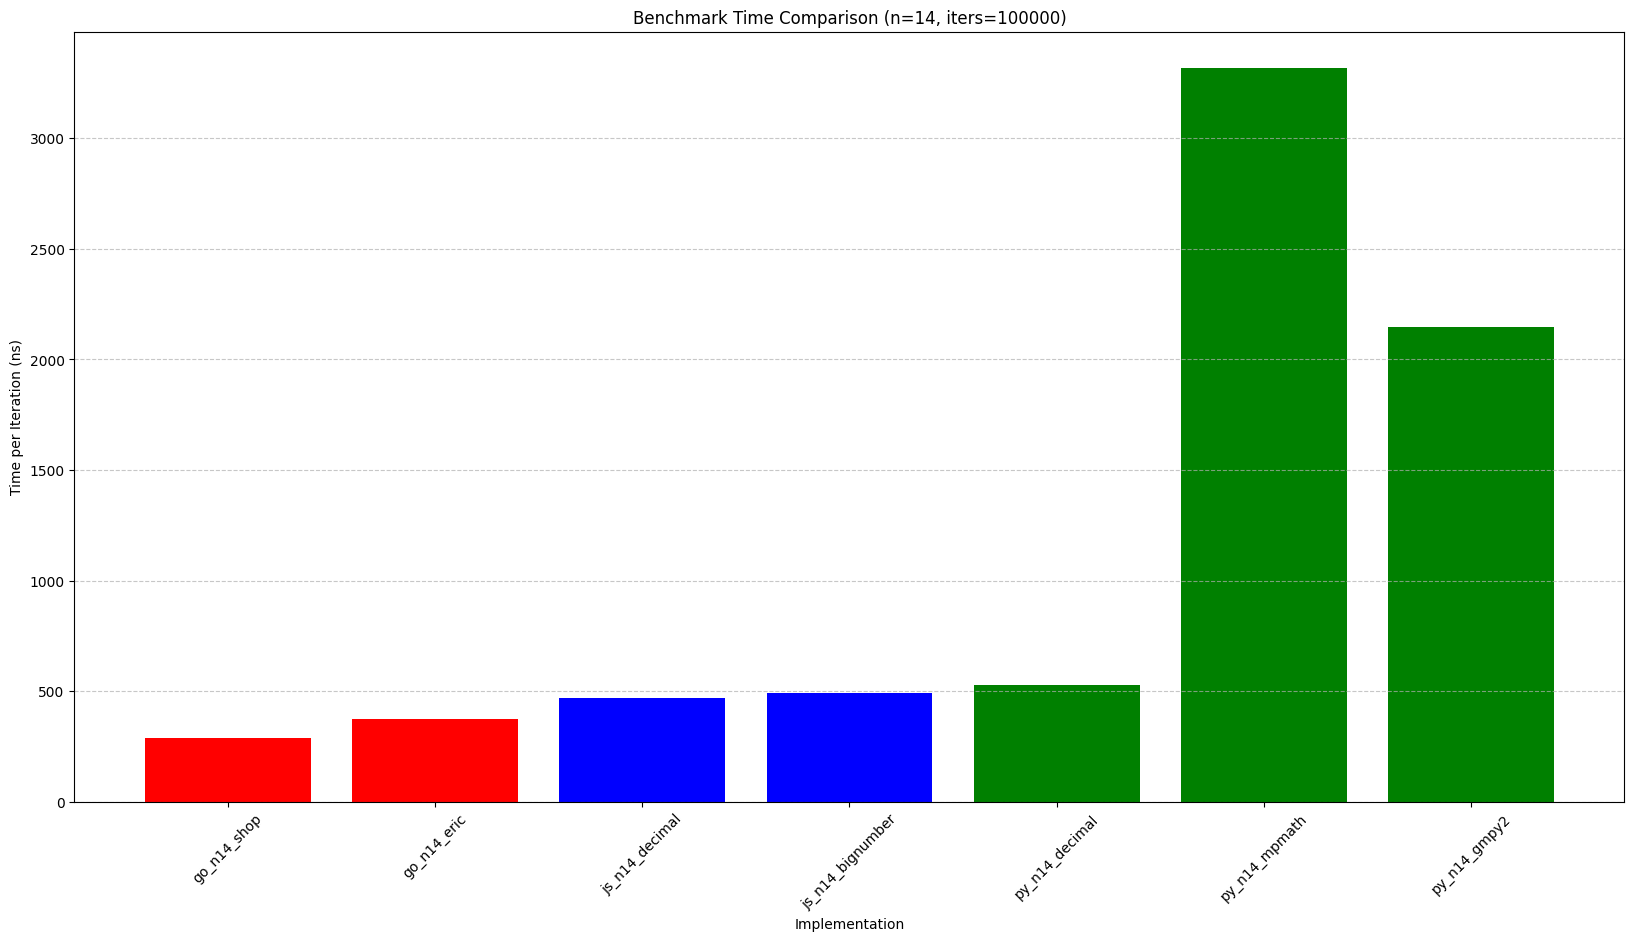
\includegraphics[width=0.75\textwidth]{images/n_14_100000.png}
    \caption{Kết quả benchmark với \( n = 10^{14} \) và vòng lặp = 100000}
    \label{fig:bench_n_14}
\end{figure}

\subsubsection{Trường hợp 2: \( n = 10^{26} \)}
\begin{figure}[h]
    \centering
    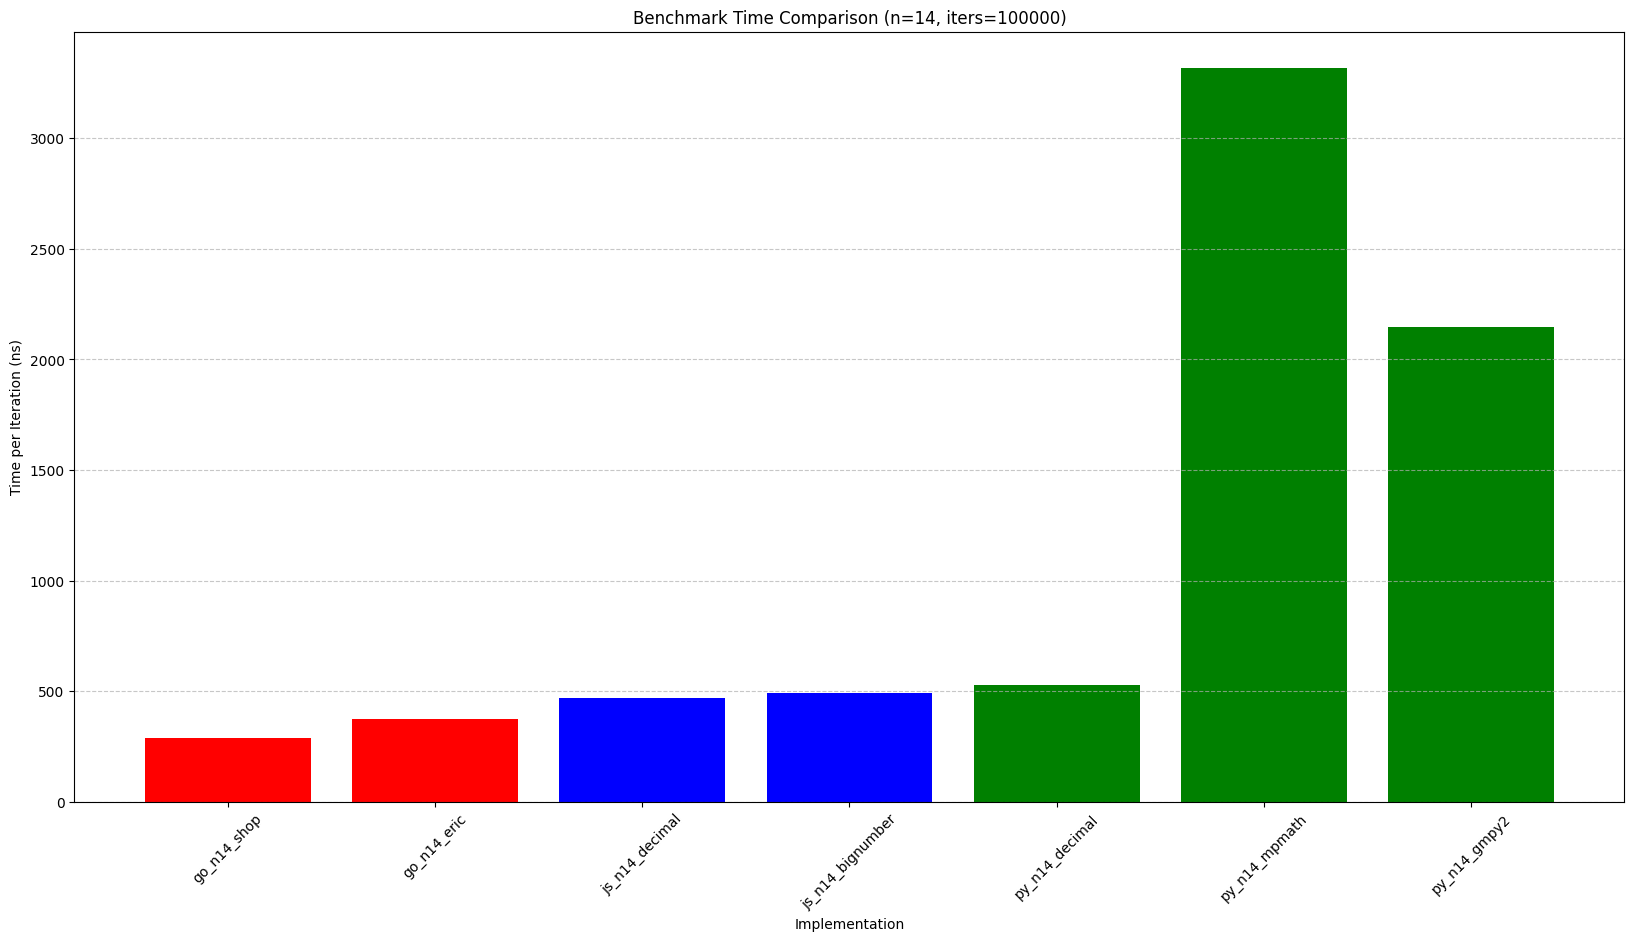
\includegraphics[width=0.75\textwidth]{images/n_14_100000.png} % Lưu ý: cần thay bằng ảnh đúng (n_26_100000.png)
    \caption{Kết quả benchmark với \( n = 10^{26} \) và vòng lặp = 100000}
    \label{fig:bench_n_26}
\end{figure}

\subsubsection{Trường hợp 3: Số nguyên lớn}
\begin{figure}[h]
    \centering
    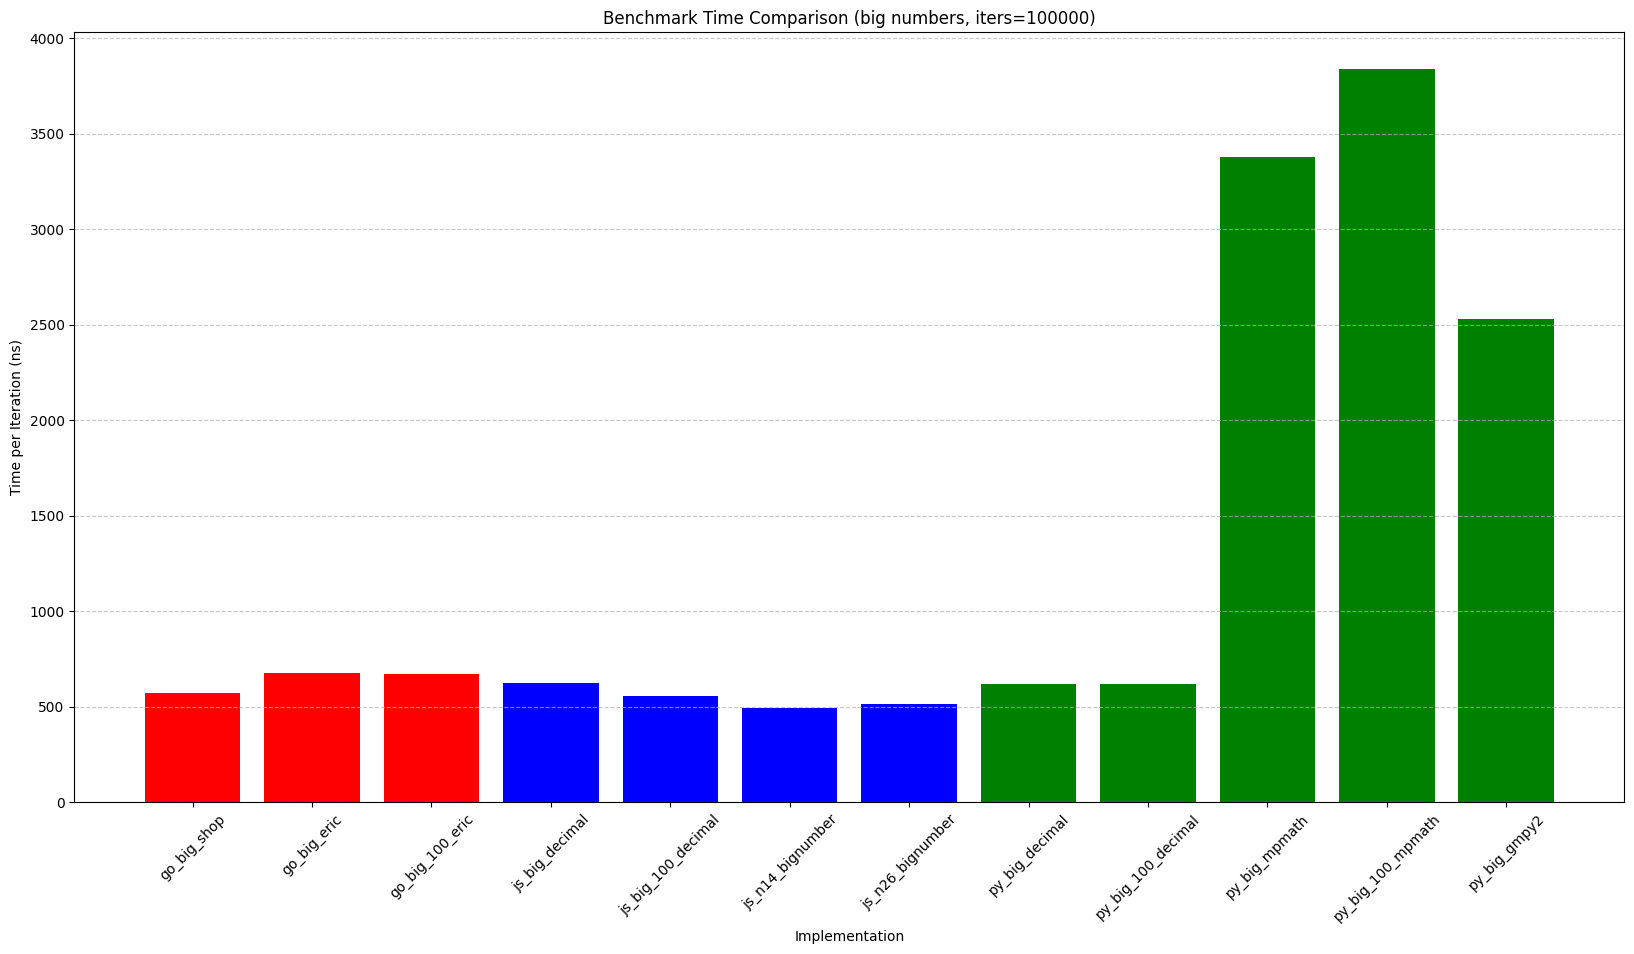
\includegraphics[width=0.7\textwidth]{images/big_100000.png}
    \caption{Kết quả benchmark với số nguyên lớn và vòng lặp = 100000}
    \label{fig:bench_big}
\end{figure}

\subsection{Phân tích kết quả}
Qua các biểu đồ \figurename{\ref{fig:bench_n_14}}, \figurename{\ref{fig:bench_n_26}} và \figurename{\ref{fig:bench_big}}, ta nhận thấy:
\begin{itemize}
    \item Các thư viện của Javascript (\texttt{decimal.js}, \texttt{bignumber.js}) và Golang (\texttt{ericlagergren/decimal}, \texttt{shopspring/decimal}) có hiệu suất tốt hơn so với Python (\texttt{decimal}, \texttt{gmpy2}, \texttt{mpmath}).
    \item Khi thay đổi hệ số precision (ví dụ: \texttt{go\_big\_100\_eric}, \texttt{js\_big\_100\_decimal}), thời gian thực thi tăng lên đáng kể, đặc biệt trong các trường hợp số lớn.
\end{itemize}

\subsection{Kết luận}
Các thư viện của Javascript và Golang phù hợp hơn cho các ứng dụng yêu cầu tính toán nhanh với số lớn, trong khi Python phù hợp hơn cho các phép tính cần độ chính xác cao nhưng không ưu tiên tốc độ.